\section{Tuning of parameters}

løn parametre

Jeg har brugt lons20 til at finde en distribution af lønnen, på tværs af alder.
Jeg har brugt lons50 til at finde trenden for lønniveauet betinget på alderen.

Jeg vil bruge dette data til at tune parametrene som styrer løn-niveau processen i modellen.

\iffalse
\begin{table}[ht]
    \centering
    \begin{tabular}{lrrrr}
\toprule
{} &    mean &    std &  skew &  kurtosis \\
gender &         &        &       &           \\
\midrule
male   &  237.54 &  38.57 & -0.44 &      0.21 \\
female &  213.31 &  33.38 &  0.56 &      1.34 \\
\bottomrule
\end{tabular}

    \caption{Wage distribution moments}
    \label{tab:my_label}
\end{table}


\begin{table}[ht]
    \centering
    \begin{tabular}{lrr}
\toprule
{} &  total obs count &  nan count \\
gender &                  &            \\
\midrule
male   &              601 &        306 \\
female &              601 &        367 \\
\bottomrule
\end{tabular}

    \caption{Wage distribution summary}
    \label{tab:my_label}
\end{table}

\begin{figure}
    \centering
    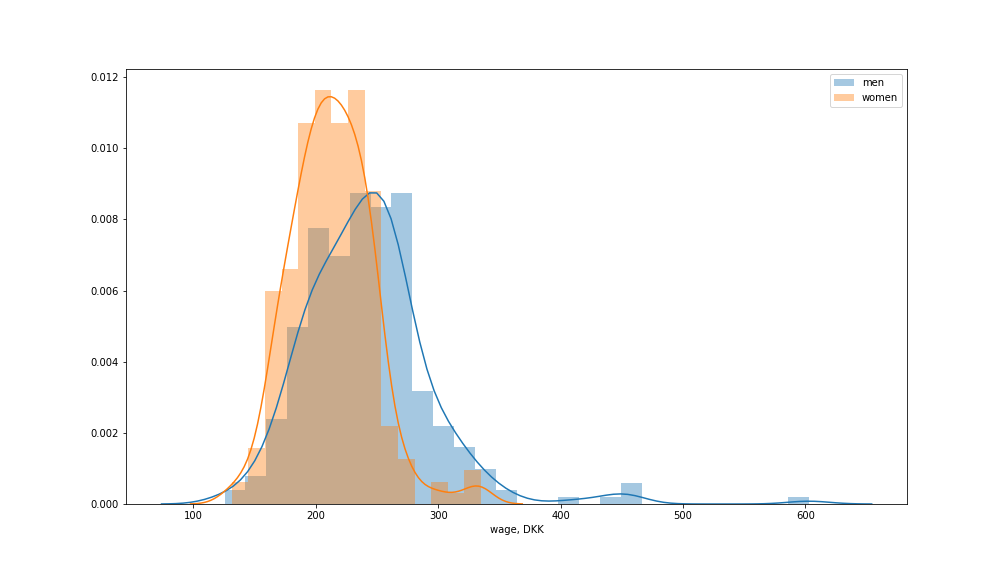
\includegraphics[scale=0.4]{figures/wage_distribution_lons20.png}
    \caption{Wage Distribution Men \& Women}
    \label{fig:my_label}
\end{figure}


\begin{figure}
    \centering
    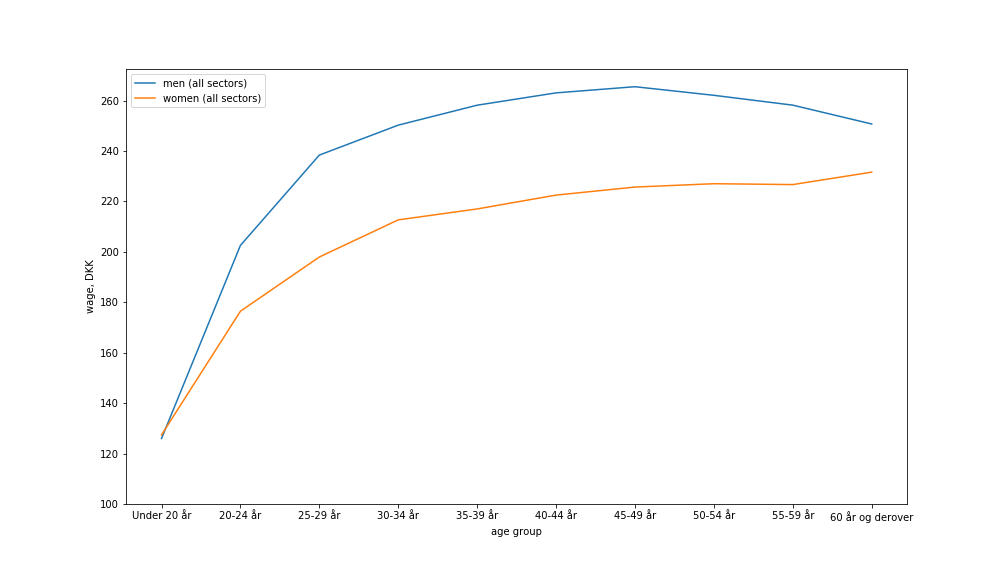
\includegraphics[scale=0.4]{figures/wage_trend_lons50.png}
    \caption{Wage Trend Men \& Women}
    \label{fig:my_label}
\end{figure}

\begin{figure}
    \centering
    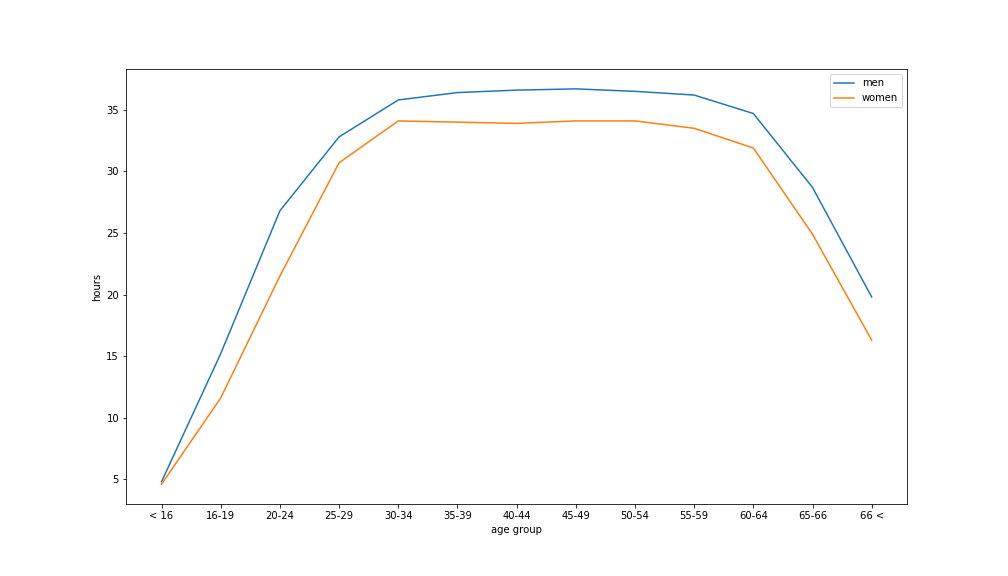
\includegraphics[scale=0.4]{figures/men_vs_women_hours_empirical.png}
    \caption{Working hours by age group (Men \& Women)}
    \label{fig:women_vs_men_hours_emmpirical}
\end{figure}

\begin{figure}
    \centering
    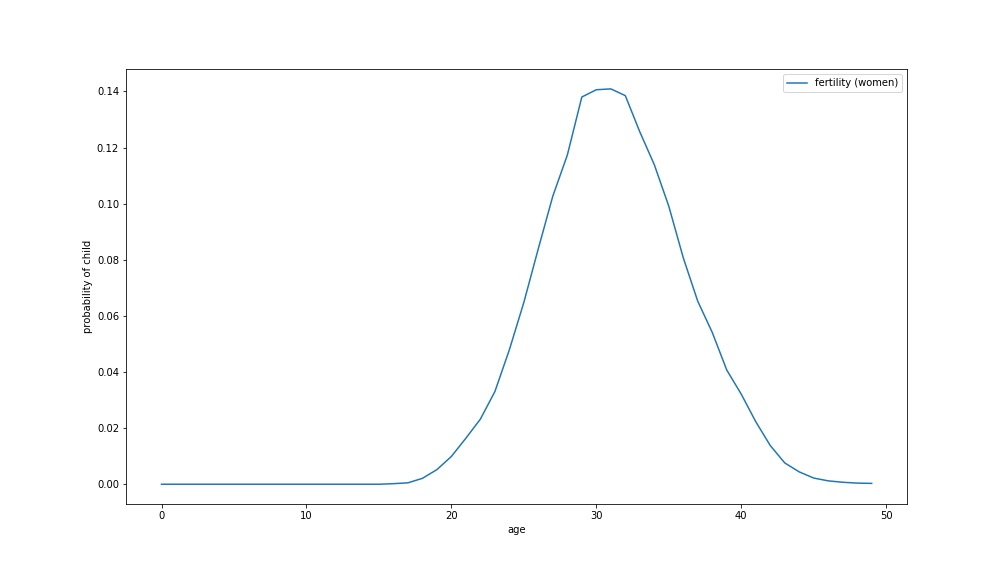
\includegraphics[scale=0.4]{figures/fertility_women_empirical.png}
    \caption{Fertility of women}
    \label{fig:fertility_by_women}
\end{figure}

\begin{figure}
    \centering
    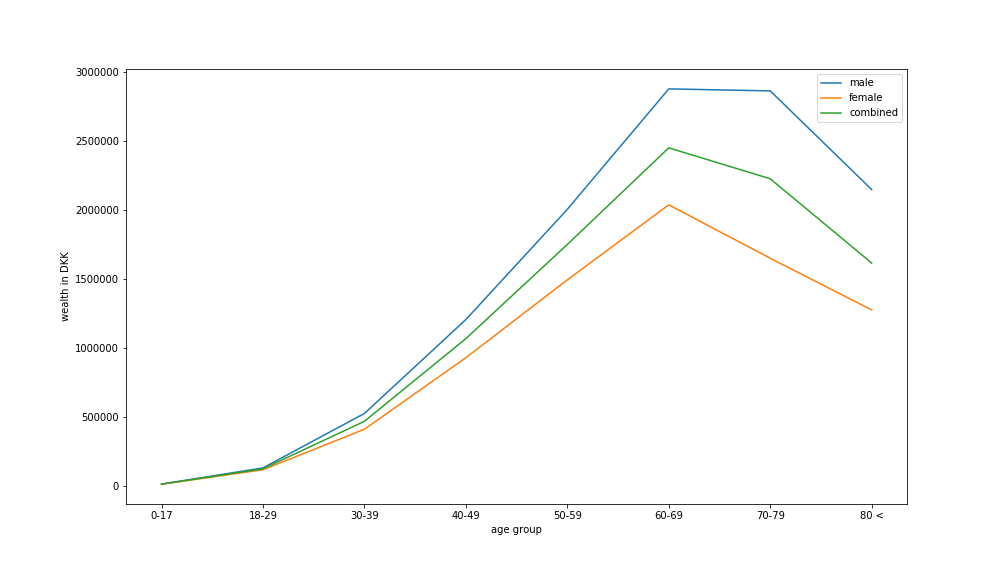
\includegraphics[scale=0.4]{figures/wealth_by_age_group_empirical.png}
    \caption{Wealth by age group}
    \label{fig:wealth_by_age_group_empirical}
\end{figure}
\fi

\subsection{Tuning the Wage process}

To solve the model i will need some initial reasonable numbers for the parameters of the wage process. The wage process contains the following parameters: $(\eta_G, \eta_{G^2}, \delta, \alpha, \sigma_{\epsilon})$. As mentioned in the model specification in section \ref{sec:model1} i specify a wage process that follow the Mincer earnings equation, where i do not account for education (this is not part of the state space), and where the idiosyncratic wage path is added linearly to the wage. I assume that the parameters driving the wage process are the same for both men and women, and these can be by tuned independent of the entire model. This is primarily due to computational constraint, since tuning multiple parameters in the same time suffers from the \textit{curse of dimensionality}. Another reason is that the wage of the husband in the model is assumed perfectly deterministic, which imply I am not able to tune the parameters driving the wage path under the assumption these are the same for men and women. As mentioned in the model specification allowing for linearly added idiosyncratic wage path that follows a random walk, allows for tuning $(\eta_G, \eta_{G^2}, \delta, \alpha)$ that drives the age and sex specific expected wage level (referred to as \textit{wage path}), while tuning the variance at each point in time can be tuned by $\sigma_\epsilon$ (referred to as \textit{wage variance}). In other words the parameter tuning of the wage process is broken into two phases: First tuning age and sex specific expected wage level, second tuning the variance of the wages.

I tune the wage path by using a \textbf{LONS50}, a data set from Statistics Denmark (Danmarks Statistik Bank). This data set contains the wage trend for men and women at any given age. My objective is to minimize the squared difference between this wage path and a predicted wage path by simulating from the partial model with given parameters and taking the average wage path. Certain things should be noted about this partial model. The wage path is a function of human capital which is the choice variable of the model specified in section \ref{sec:model1}. This obviously makes it problematic to tune the parameters. I work around the problem by using the data set \textbf{LIGEF15} containing the number of worked hours for both men and women, which is supplied by Statistics Denmark. Since these numbers do not take into account people leaving the labour force temporarily - which we know women to do when giving birth. I model this the following way. I assume that women leave the work force for 1 year when giving birth to a child. I use the data set \textbf{FOD33} to get fertility rates of women. Again this data is supplied by Statistics Denmark. Formally this can summed up to:

\begin{equation}
    H_t = \begin{cases}
        H^{men}(Q) & \text{if sex=\textit{male}} \\
        H^{women}(Q) & \text{if sex=\textit{female} and birth=\textit{false}} \\
        0 & \text{if sex=\textit{female} and birth=\textit{true} }\\
    \end{cases}    
\end{equation}

The rest of the wage process follows the model described in section \ref{sec:model1}. The minimization problem follows the following process:

\begin{equation}
    \text{Cohort Average: } {\tilde{\mu}}_i (C_i) = \frac{1}{\mid C_i \mid} \sum_{\tilde{w}_{n, q} \in C_i} {\tilde{w}_{n, q}}
\end{equation}

\begin{equation}
    \underset{\hat{\eta_G}, \hat{\eta_{G^2}}, \hat{\delta}, \hat{\alpha}}{\argmin} = \frac{1}{2}\frac{1}{\mid C \mid } \sum_{C_i \in C} \lp\lp \mu_{i}^{men}(C_i)  - \tilde{\mu}_i^{men}(C_i)\rp^2 + \lp \mu_{i}^{women}(C_i)  - \tilde{\mu}_i^{women}(C_i)\rp^2 \rp
\end{equation}

where $\tilde{w}_{n, q}$ denotes a simulated wage at age $q$ for the $n'tn$ simulated individual and $w_q$ is the true value wage level for a given age. $C_i \in C$ denotes a given age cohort, where the age cohorts are $C=\{(20, 24), (25, 29), \cdots , (55, 59) \}$. $\mu_i$ denotes the empircal average for a given cohort.
I solve the minimization problem using Nelder-Mead (Simplex method). Essentially The simplex method allows for numerical optimization without the need to supply neither the gradient, Hessian or Jacobian matrix. I initialize the algorithm with the values: $(\alpha=4, \eta_G = 0.5, \eta_{G^2}=0.01, \delta=0.5)$, and let the algorithm run for a maximum of 100 iterations. 

Given the now tuned parameters driving the wage path, only a single parameter $\sigma_\epsilon$ needs to be tuned. This is again done by numerical optimization. This is done by minimizing the mean squared error between the empirical quartiles (upper and lower) for men and women, to those found by simulating for the given parameters:

\begin{equation}
    \text{Cohort Quartile: } {\tilde{\omega}}_{i, j} (C_i) = \text{quartile}_j (C_i), \qquad j\in{\text{upper}, \text{lower}} 
\end{equation}

\begin{equation}\label{eq:wage_var_optimization}
    \underset{\hat{\sigma_\epsilon}}{\argmin} = \frac{1}{2}\frac{1}{2}\frac{1}{\mid C \mid } \sum_{j} \sum_{sex}\sum_{C_i} \lp \omega_{i, j}^{sex}(C_i)  - \tilde{\omega}_{i,j}^{sex}(C_i)\rp^2, \qquad 
\end{equation}

Where equation \eqref{eq:wage_var_optimization} assummes $C_i \in C$, $j \in \{\text{upper},  \text{lower} \}$, and $sex \in \{\text{men}, \text{women} \}$. Again i use Nelder-Mead for optimization, set a max number of iterations at 100, and lastly i let the starting value of $\sigma_\epsilon = 0.5$. Below are the results of the optimized parameters listed in table \ref{tab:wage_path_optimized_params}:

\begin{table}[ht]
    \centering
    \begin{tabular}{lrrrrr}
\toprule
{} &  $\hat{\alpha}$ &  $\hat{\eta_G}$ &  $\hat{\eta_{G^{2}}}$ &  $\hat{\delta}$ &  $\hat{\sigma_{\epsilon}}$ \\
\midrule
Parameters &           4.609 &           0.164 &                 0.015 &           0.209 &                      15.11 \\
\bottomrule
\end{tabular}

    \caption{Optimized parameters for wage process}
    \label{tab:wage_path_optimized_params}
\end{table}

KOMMENTER PÅ RESULTATERNE SAMMENLIGNET MED LITTERATUREN. 

\begin{figure}[ht]

% NOTE THAT I HAVE INTERCHAGNED THE NAME OF MEN AND WOMEN
\begin{subfigure}{.5\textwidth}
  \centering
  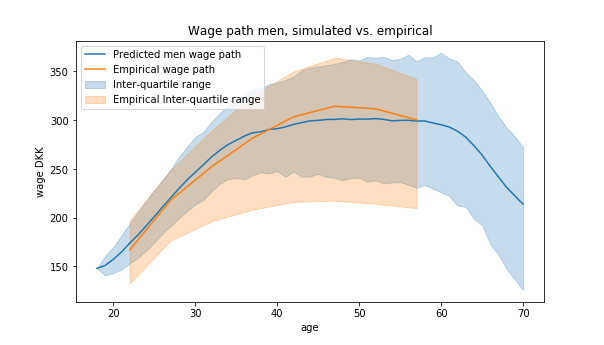
\includegraphics[width=1\linewidth]{figures/simulated_wage_path_variance_optimized_parameters_women.png}
  \caption{Men}
  \label{fig:sub1}
\end{subfigure}%
\begin{subfigure}{.5\textwidth}
  \centering
  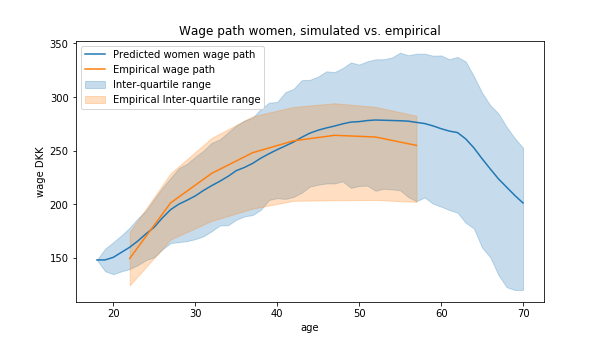
\includegraphics[width=1\linewidth]{figures/simulated_wage_path_variance_optimized_parameters_men.png}
  \caption{Women}
  \label{fig:sub2_wage_path}
\end{subfigure}
    \caption{Simulated wage process vs Empirical wage process}
    \label{fig:sim_wage_vs_empirical_wage}
\end{figure}

Figure \ref{fig:sim_wage_vs_empirical_wage} allows for comparing the empirical wage process with the simulated. First looking to the \textit{wage path}, I conclude that the mincer equation (even though it does not account for education level), seem to give a relatively good fit to the data even without taking education into account, and even though it's assumed that the parameters driving the wage process are the same. The mean absolute error for the women wage path is $10.61$ DKK, and for men the number is $5.84$ DKK, which considering the relatively simple parametric form of the process, is very good. Considering the variance of the wage process, it should be noted that the empirical wage process is skewed. In this setup, this is not the case. This is, however, a consequence of the design of the wage process, yielding it easier to tune. It should be noted that the size of the inter-quartile range seem to fit the wage path of men reasonably, but for women it slighty overshoots.

\subsection{Initial parameter values for the utility function}

SKAL SKRIVES OM!!!

We see in equation \eqref{eq:utility_v1} that drives the utility function three parameters are present: $\beta_K, \beta_L, \beta_Y$. As mentioned i restrict $\beta_Y = 1$ to achieve identification, over the latent variables. Now since it can be computationally heavy to solve the model using simulation and indirect inference, some initial values of $\beta_K, \beta_L$ needs to be found, that will give a reasonable fit to the model when solving. I create an agent that moves in some reasonable fashion to create a initial fit of the model. Again I will stress, that these values are not by any means optimal, they are however a good starting point.

The agent moves by the following metric:

\begin{equation}
    H_t = \begin{cases}
        H^{women}(Q) & \text{if } K\leq 2 \\
        0 & \text{else } 
    \end{cases}
\end{equation}

Now I can write up the optimzation needed to be performed:

\begin{equation}
    \underset{\beta_K, \beta_L}{\argmax} = \frac{1}{N} \sum_{i=1}^{N}  \sum_{t } U_{t, i} 
\end{equation}

Where here $N$ denotes the number of simulated agents and $t$ denotes the timestep. $U_{t,i}$ is the utility of a given agent at a given timestep. In other words the optimization problem trying to be solved is: